% A dissertation in the classicthesis style (André Miede): Palatino, small-caps headings, a
% generous margin for short notes. The class is KOMA-Script's scrbook; the look comes from the
% classicthesis package, set up in classicthesis-config.tex (the way its own manual recommends).
\documentclass[
  twoside, openright, titlepage, numbers=noenddot,
  headinclude, footinclude=true, cleardoublepage=empty,
  BCOR=5mm, paper=a4, fontsize=11pt, american
]{scrbook}

\usepackage[T1]{fontenc}
\usepackage[utf8]{inputenc}
\usepackage[american]{babel}
\usepackage[dvipsnames]{xcolor}   % classicthesis needs the dvips colour names
\usepackage{graphicx}
\usepackage{amsmath}
% Author-year citations with BibTeX; classicthesis loads hyperref itself, so natbib goes first.
\usepackage[round,authoryear]{natbib}
\usepackage{tikz}
\usetikzlibrary{arrows.meta,positioning}

% Everything you set once for the whole thesis.

% --- Your details: used on the title page and in the PDF properties. ---
\newcommand{\myTitle}{A Clear Title That Says What the Thesis Is About}
\newcommand{\mySubtitle}{An optional subtitle, or delete it}
\newcommand{\myName}{Your Name}
\newcommand{\myDegree}{Doctor of Philosophy}
\newcommand{\myProf}{Prof.\ Dr.\ Supervisor Name}
\newcommand{\myUni}{Example University}
\newcommand{\myFaculty}{Faculty of Science}
\newcommand{\myTime}{March 2026}

% --- classicthesis options. ---
% style=classicthesis is the default look; arsclassica, linedheaders and plain are alternatives.
% dottedtoc: dotted leaders between contents entries and page numbers.
% eulerchapternumbers: chapter numbers in the Euler face instead of Palatino.
% eulermath: Euler for formulas as well (a matter of taste: remove it for plain Palatino maths).
% drafting (add it while writing): prints the compile date in the footer of every page.
\usepackage[
  style=classicthesis, dottedtoc, eulerchapternumbers, eulermath
]{classicthesis}

% PDF title and author. classicthesis has already loaded hyperref with coloured links
% (green citations, blue links); add `hidelinks` inside \hypersetup for a print version.
\hypersetup{pdftitle={\myTitle}, pdfauthor={\myName}}

% cleveref (\cref) must come after hyperref, so it is loaded here rather than in main.tex.
\usepackage[nameinlink]{cleveref}
   % title, author, and the classicthesis options

\begin{document}
\frenchspacing
\raggedbottom
\pagenumbering{roman}
\pagestyle{plain}

\begin{titlepage}
  \pdfbookmark[1]{\myTitle}{titlepage}
  \begin{center}
    \large
    \hfill\vfill
    \begingroup
      \color{CTtitle}\spacedallcaps{\myTitle} \\ \bigskip
      \spacedlowsmallcaps{\mySubtitle}
    \endgroup
    \vfill
    \spacedlowsmallcaps{\myName}
    \vfill
    Dissertation submitted for the degree of \\
    \myDegree \\[1ex]
    \myFaculty \\
    \myUni \\[2ex]
    \myProf \\[2ex]
    \myTime
    \vfill\vfill
  \end{center}
\end{titlepage}

% Optional: an imprint page on the back of the title page with the exact reference.
\thispagestyle{empty}
\hfill\vfill
\noindent\myName: \textit{\myTitle}, \myDegree, \textcopyright\ \myTime.

\pdfbookmark[1]{Abstract}{Abstract}
\chapter*{Abstract}
% One page at most: the question, the method, the main findings and why they matter.
% Write it last, in the present tense, and make it readable without the rest of the thesis.
State the problem this dissertation addresses and why it is hard. Say in a sentence or two
what you did, then the main results with one or two numbers if you have them, and close
with what the work changes for the field.

\cleardoublepage
\pdfbookmark[1]{Acknowledgments}{acknowledgments}
\chapter*{Acknowledgments}
% Thank your supervisor, colleagues, funders, family and friends. Keep it short and sincere.
I thank my supervisor for guidance and patience, my colleagues for many good discussions, and
the funding bodies that made this work possible. Last, my thanks to family and friends for
their support.


\pagestyle{scrheadings}
\tableofcontents
\listoffigures
\listoftables

\cleardoublepage
\pagenumbering{arabic}

% One file per chapter: \include starts a new page and lets you rebuild just one chapter.
\chapter{Introduction}\label{ch:introduction}

\section{Motivation}
Why is this topic important? Start broad and narrow down to your question within a page.
Cite sources with \texttt{\textbackslash citet} in the sentence, as \citet{knuth84} does,
or in parentheses with \texttt{\textbackslash citep} \citep{lamport94}.
\graffito{Short notes, definitions and pointers go in the margin with \texttt{\textbackslash graffito}.}

\section{Research Questions}
State the questions the thesis answers, preferably as a short numbered list.
\begin{enumerate}
  \item What is the first question?
  \item What is the second question?
\end{enumerate}

\section{Contributions and Outline}
List what is new in this work, then summarize each chapter in a sentence:
\cref{ch:method} describes the method, \cref{ch:results} reports the results and
\cref{ch:conclusion} concludes.

\paragraph{Notation.} Subsections and paragraph headings are set in small caps as well, so
the hierarchy stays calm even in long chapters.

\chapter{Method}\label{ch:method}

\section{Overview}
Describe the approach so that someone could repeat it. A diagram often says it faster than
a paragraph; \cref{fig:pipeline} is drawn with TikZ, so it needs no image file.

\begin{figure}[bth]
  \centering
  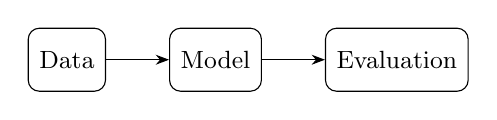
\begin{tikzpicture}[node distance=8mm, box/.style={draw, rounded corners, minimum height=8mm, inner sep=4pt, font=\small}]
    \node[box] (data) {Data};
    \node[box, right=of data] (model) {Model};
    \node[box, right=of model] (eval) {Evaluation};
    \draw[-{Stealth}] (data) -- (model);
    \draw[-{Stealth}] (model) -- (eval);
  \end{tikzpicture}
  \caption[Short title for the list of figures]{The pipeline in three steps. Keep captions
    short and self-contained.}\label{fig:pipeline}
\end{figure}

\section{Formal Setting}
Number only the equations you refer to later. For example, the objective in
\cref{eq:objective} is minimized over the parameters $\theta$:
\begin{equation}\label{eq:objective}
  \hat{\theta} = \operatorname*{arg\,min}_{\theta}\; \frac{1}{n}\sum_{i=1}^{n} \ell\bigl(f_\theta(x_i), y_i\bigr) + \lambda\,\lVert\theta\rVert^2 .
\end{equation}

\chapter{Results}\label{ch:results}

\section{Main Findings}
Report what you found before interpreting it. \Cref{tab:results} uses the \texttt{booktabs}
rules that classicthesis already loads: horizontal rules only, no vertical lines.

\begin{table}[bth]
  \centering
  \caption[Short title for the list of tables]{Results on the test set (mean over five runs).}\label{tab:results}
  \begin{tabular}{@{}lrr@{}}
    \toprule
    Method & Accuracy (\%) & Time (s) \\
    \midrule
    Baseline & 81.2 & 12 \\
    Our method & 86.9 & 15 \\
    \bottomrule
  \end{tabular}
\end{table}

\section{Discussion}
Interpret the numbers: what do they show, what do they not show, and where could the
result be misleading?

\chapter{Conclusion}\label{ch:conclusion}

\section{Summary}
Answer the research questions from \cref{ch:introduction} one by one, in the same order.

\section{Limitations and Future Work}
Say honestly what the work does not cover, and which questions it opens.


\appendix
\chapter{Supplementary Material}\label{app:supplement}
Proofs, long tables, questionnaires and anything else that would interrupt the argument
in the main text. After \texttt{\textbackslash appendix}, chapters are numbered A, B, C.


\backmatter
\cleardoublepage
\bibliographystyle{plainnat}
\bibliography{refs}

\end{document}
